\section{Valid inequalities}

In this chapter, we will discuss the idea of generating and adding constraints to improve a formulation of a (possibly mixed-)integer programming problem. This idea can either be implemented in a priori setting, for example before employing the branch-and-bound method, or as the solution method itself. These constraints are often called \emph{valid inequalities} or \emph{cuts}, though the latter is typically used in the context of cutting-planes methods.

Let us start by defining the integer programming problem
%
\begin{equation*}
	(IP) : \maxi_x \braces{c^\top x : x \in X}
\end{equation*}
%
where $X = P \cap \integers^n$ and $P = \braces{x \in \reals^n : Ax \leq b, x \geq 0}$, with $A \in \reals^{m \times n}$ and $b \in \reals^m$. 

The idea of using constraints to solve $IP$ is founded in the following observations. We know that $\conv(X)$ is a (convex) polyhedral set (cf. Definition \ref{p1c2:def:convex_combination_hull}) and, being so, there exists a finite set of inequalities $\tilde{A}x \le \tilde{b}$ such that 
%
\begin{equation*}
	\conv(X) = \braces{x \in \reals^n: \tilde{A}x \leq \tilde{b}, x \geq 0}	
\end{equation*}
%
Furthermore, if we had available $\tilde{A}x \le \tilde{b}$, then we could solve $IP$ by solving its linear programming relaxation.

Cutting-plane methods are based on the idea of iteratively approximating the set of inequalities $\tilde{A}x \le \tilde{b}$ by adding constraints to the formulation $P$ of $IP$. These constraints are called \emph{valid inequalities}, a term we define more precisely in Definition \ref{p1c10:def:valid_inequality}.

\begin{definition}[Valid inequality] \label{p1c10:def:valid_inequality}
	An inequality $\pi^\top  x \leq \pi_0$ is valid for $X \subset \reals^n$ if $\pi^\top  x \leq \pi_0$ for all $x \in X$.
\end{definition}

Notice that the condition for an inequality to be valid is that it does not remove any of the point in the original integer set $X$. In light of the idea of gradually approximating $\conv(X)$, one can infer that good valid inequalities are those that can ``cut off'' some of the area defined by the polyhedral set $P$, but without removing any of the points in $X$. This is precisely where the name \emph{cut} comes from. Figure \ref{p1c10:fig:valid_inequality} illustrates the process of adding a valid inequality to a formulation $P$. Notice how the inequality expose one of the facets of the convex hull of $X$. Cuts like such are called ``facet-defining'' and are the strongest types of cuts one can generate. We will postpone the discussion of stronger cuts to later in this chapter.

\begin{figure}
	\centering
	\begin{subfigure}{0.49\textwidth}
		\centering
		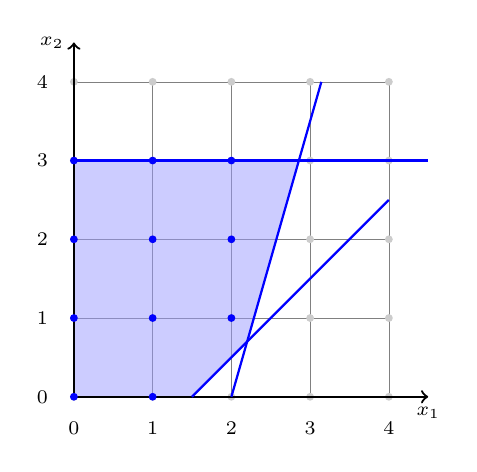
\begin{tikzpicture}[scale = 1,
		point/.style={circle, fill=gray!40, inner sep=1pt},
		feas point/.style={circle, fill=blue, inner sep=1pt}]
			\draw[help lines] (0,0) grid (4,4);  
			\fill[blue!40, opacity=0.5] (0,0) -- (1.5, 0) -- (2.2, 0.7) --(20/7, 3) -- (0,3);          
			\foreach \x in {0,...,4}{
			  \foreach \y in {0,...,4} {
			      \node[point] (\x,\y) at (\x, \y) {};
			  }}
			\foreach \x in {0,...,4}{
			  \node[font=\scriptsize] at (\x,-0.4) {$\x$};
			}
			\foreach \y in {0,...,4}{
			  \node[font=\scriptsize] at (-0.4,\y) {$\y$};
			}                      
			\draw[thick, <->] (4.5,0) node[below, font=\scriptsize]{$x_1$} -- (0,0) -- (0,4.5) node[left, font=\scriptsize]{$x_2$};    
			\draw[domain=0:4.5, thick, variable=\x, blue] plot (\x,{3});
			\draw[domain=2:22/7, thick, variable=\x, blue] plot (\x,{-14/2 + 7/2*\x});
			\draw[domain=1.5:4, thick,variable=\x,blue] plot ({\x},{-3/2 + \x});
			\node[feas point] at (0,0){};
			\node[feas point] at (1,0){};
			\foreach \x in {0,...,2}{ 
			  \foreach \y in {1,...,3}{        
			      \node[feas point] at (\x,\y){};
			}}
		\end{tikzpicture}	
	\end{subfigure}
	\hfill
	\begin{subfigure}{0.49\textwidth}
		\centering
		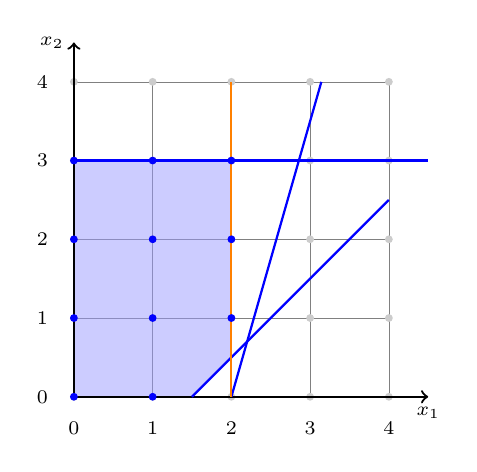
\begin{tikzpicture}[scale = 1,
		point/.style={circle, fill=gray!40, inner sep=1pt},
		feas point/.style={circle, fill=blue, inner sep=1pt}]
			\draw[help lines] (0,0) grid (4,4);  
			\fill[blue!40, opacity=0.5] (0,0) -- (1.5, 0) -- (2, 0.5) --(2, 3) -- (0,3);          
			\foreach \x in {0,...,4}{
			  \foreach \y in {0,...,4} {
			      \node[point] (\x,\y) at (\x, \y) {};
			  }}
			\foreach \x in {0,...,4}{
			  \node[font=\scriptsize] at (\x,-0.4) {$\x$};
			}
			\foreach \y in {0,...,4}{
			  \node[font=\scriptsize] at (-0.4,\y) {$\y$};
			}                      
			\draw[thick, <->] (4.5,0) node[below, font=\scriptsize]{$x_1$} -- (0,0) -- (0,4.5) node[left, font=\scriptsize]{$x_2$};    
			\draw[domain=0:4.5, thick, variable=\x, blue] plot (\x,{3});
			\draw[domain=2:22/7, thick, variable=\x, blue] plot (\x,{-14/2 + 7/2*\x});
			\draw[domain=1.5:4, thick,variable=\x,blue] plot ({\x},{-3/2 + \x});
			\draw[orange, thick] (2,0) -- (2,4);
			\node[feas point] at (0,0){};
			\node[feas point] at (1,0){};
			\foreach \x in {0,...,2}{ 
			  \foreach \y in {1,...,3}{        
			      \node[feas point] at (\x,\y){};
			}}
		\end{tikzpicture}	
	\end{subfigure}
	\caption{Illustration of a valid inequality being added to a formulation $P$. Notice how the inequality cuts of a portion of the polyhedral set $P$ while not removing any of the feasible points $X$ (represented by the dots)} \label{p1c10:fig:valid_inequality}
\end{figure}


\section{The Chv\'atal-Gomory procedure}

To develop a systematic procedure for generating valid inequalities in the context of a solution method for integer programming problems, we will rely on a two step procedure. First, a cut that is valid for the polyhedral set $P$ is (somewhat automatically) generated, and then it is made valid for the integer set $X$ by a simple rounding procedure. Before we proceed, let us define the notion of valid inequalities in the context of linear programming problems.

\begin{proposition}[Valid inequalities for polyhedral sets] \label{p1c10:prop:valid_inequality_LP}
	An inequality $\pi^\top x \leq \pi_0$ is valid for $P = \braces{x \in \reals^n : Ax \leq b, x \geq 0}$, if and only if $P \neq \emptyset$ and there exists $u \geq 0$ such that $u^\top A \geq \pi$ and $u^\top b \leq \pi_0$.
\end{proposition}

\begin{proof}
	We can use linear programming duality to prove this statement. First, notice that, if the proposition holds, for $u \ge 0$ and $x \in P$, we have 
	%
	\begin{align*}
		Ax & \le b \\
		u^\top Ax & \le u^\top b \\
		\pi ^\top x \le u^\top Ax & \le u^\top b \le \pi_0,
	\end{align*}
	%
	and, thus, it implies the validity of the cut, i.e., that $\pi^\top x \leq \pi_0, \forall x \in P$. Now, consider the primal problem
	%
	\begin{align*}
		\maxi & \pi ^\top x \\
		\st   & Ax \leq b \\
		      & x \geq 0
	\end{align*}
	%
	and its dual 
	%
	\begin{align*}
		\mini & u^\top b \\
		\st   & u^\top A \geq \pi \\
		      & u \geq 0. 
	\end{align*}
	%
	Thus, $u^\top A\geq \pi$ can be seen as a consequence of dual feasibility, which is guaranteed to hold for some $u$ since $\pi^\top x$ is bounded. Furthermore, strong duality gives $u^\top b = \pi ^\top x \leq \pi_0$, completing the proof. 
\end{proof}

One thing to notice is that valid cuts in the context of polyhedral sets are somewhat redundant, since, by definition, they do not alter the polyhedral set in any means. However, the concept can be combined with a simple yet powerful way of generating valid inequalities for integer set by using rounding. This is stated in Proposition \ref{p1c10:prop:valid_inequality_IP}. 
%
\begin{proposition}[Valid inequalities for integer sets] \label{p1c10:prop:valid_inequality_IP}
	Let $X = \braces{y \in \integers^1 : y \leq b}$. The inequality $y \leq \floor{b}$ is valid for $X$.
\end{proposition}
%
The proof of Proposition \ref{p1c10:prop:valid_inequality_IP} is somewhat straightforward and left as a thought exercise. 

We can combine Propositions \ref{p1c10:prop:valid_inequality_LP} and \ref{p1c10:prop:valid_inequality_IP} into a single procedure to automatically generate valid inequalities. Let us start with a numerical example. Consider the set $X = P \cap \integers^n$ where $P$ is defined by
	%
	\begin{equation*}
		P = \braces{x \in \reals^2_+ : 7x_1 -2x_2 \leq 14, x_2 \leq 3, 2x_1 - 2x_2 \leq 3}.
	\end{equation*}
	
First, let $u=\left[\frac{2}{7}, \frac{37}{63}, 0\right]$, which, for now, we can assume that they were arbitrarily chosen. We can then combine the constraints in $P$ (the $Ax \le b$ in Proposition \ref{p1c10:prop:valid_inequality_LP}) forming the constraint (equivalent to $u^\top Ax \le u^\top b$)
	%
	\begin{equation*}
		2x_1 + \frac{1}{63}x_2 \leq \frac{121}{21}.
	\end{equation*}
	
Now, notice that the constraint would remain valid for $P$ if we simply \emph{round down} the coefficients on the lefthand side (as $x \ge 0$ and all coefficients are positive). This would lead to the new constraint (notice that this yields a vector $\pi$ in Proposition \ref{p1c10:prop:valid_inequality_LP})
	%
	\begin{equation*}
		2x_1 + 0x_2 \leq \frac{121}{21}.
	\end{equation*}
	
Finally, we can invoke Proposition \ref{p1c10:prop:valid_inequality_IP} to generate a cut valid for $X$. This can be achieved by simply rounding down the righthand side (yielding $\pi_0$), obtaining
	%
	\begin{equation*}
		2x_1 + 0x_2 \leq 5,
	\end{equation*}
	%
	which is valid for $X$, but not for $P$. Notice that, apart from the vector of weights $u$ used to combine the constraints, everything else in the procedure of generating the valid inequality for $X$ is automated. This procedure is known as the \emph{Chv\'atal-gomory procedure} and can be formalised as follows.
	
\begin{definition}[Chv\'atal-Gomory procedure] \label{p1c10:def:CG-procedure}
	Consider the integer set $X = P \cap \integers^n$ where \lb $P = \braces{x \in \reals^n_+ : Ax \leq b}$, $A$ is an $m \times n$ matrix with columns $\braces{A_1, \dots, A_n}$ and $u \in \reals^m_+$.
	
	The Chv\'atal-Gomory procedure consists of the following set of steps to generate valid inequalities for $X$:
	\begin{enumerate}
	    \item $\sum_{j=1}^n u^\top A_jx_j \leq u^\top b$ is valid for $P$ as $u\geq 0$;
	    \item $\sum_{j=1}^n \floor{u^\top A_j}x_j \leq u^\top b$ is valid for $P$ as $x \geq 0$;
	    \item $\sum_{j=1}^n  \floor{u^\top A_j}x_j \leq \floor{u^\top b}$ is valid for $X$ as LHS is integer.
	\end{enumerate}		
\end{definition}
	
Perhaps the most striking result in the theory of integer programming is that \emph{every} valid inequality for an integer set $X$ can be obtained by employing the Chv\'atal-gomory procedure a number of times. This is formalised in Theorem \ref{p1c10:thm:VG_valid_inequality}.

\begin{theorem} \label{p1c10:thm:VG_valid_inequality}
	Every valid inequality for $X$ can be obtained by applying the Chv\'atal-Gomory procedure a finite number of times.
\end{theorem}
	
% TODO: Add a reference	to the proof in the big Nemhauser and Wolsey book.
	
	
\section{The cutting-plane method}

Let us now consider how one could use valid inequalities to devise a solution method. The working paradigm behind a cutting-plane method is the \emph{separation principle}. 

The separation principle states that, given an integer set $X = P \cap \integers^n$ if a solution $x \notin X$, then there exists a hyperplane $\pi^\top x \leq \pi_0$ separating $x$ and $X$\footnote{the separation principle is a consequence of the separation theorem (Theorem \ref{p2c2:thm:separation}) in Part \ref{part_2}.}. As one might infer, the challenge is how one can generate such pairs $(\pi, \pi_0)$. This is precisely what is called the \emph{separation problem}, in the context of integer programming.

In general, these valid inequalities are generated from a family of inequalities $\mathcal{F}$, which are related to each other by properties related to, e.g., problem structure or nature of the inequality itself. One way of thinking about it is to see the family of inequalities $\mathcal{F}$ as a means to dictate, to some extent, how the selection of weights $u$ in the Chv\'atal-Gomory procedure is defined.

In any case, in possession of a family of inequalities and a method to solve the separation problem, we can pose a cutting-plane methods in general terms. This is stated in Algorithm \ref{p1c10:alg:cuting-plane}.

\begin{algorithm}[h]
	\caption{Cutting-plane algorithm} \label{p1c10:alg:cuting-plane}
	\begin{algorithmic}[1] %line numbering frequency. 
		\State {\bf initialise.} let $\mathcal{F} \subseteq \braces{(\pi, \pi_0) : \pi^\top  x \leq \pi_0 \text{ is valid for } X}$. $k \gets 0$. 
		\While {$x_{LP}^k \notin \integers^n$} \label{Alg2:loop}
		    \State solve the LP relaxation over $P$, obtaining the optimal objective value $z_{LP}^k$ and optimal solution $x_{LP}^k$. 
		    \If {$x_{LP}^k \notin \integers^n$} 
		        find $(\pi^k, \pi^k_0) \in \mathcal{F}$ such that ${\pi^k}^\top x > \pi^k_0$. \label{Alg2:SepProb}
		    \Else 
		    	\State {\bf return} ($x_{LP}^k, z_{LP}^k$).
		    \EndIf
		    \State $P \gets P \cup \braces{{\pi^k}^\top x \leq \pi^k_0}$. $k \gets k+1$.
		\EndWhile
	    \State {\bf return} ($x_{LP}^k, z_{LP}^k$).
	\end{algorithmic}
\end{algorithm}

Notice that we have already discussed a cutting-plane method before in Chapter \ref{chapter_7}, when we presented the Benders decomposition. In that case, the optimality and feasibility cuts form the family of valid inequalities $\mathcal{F}$, while the separation problem was the subproblem responsible to find the cuts that were violated by the current main problem solution. 

Like it was the case in Benders decomposition, the motivation of cutting-plane algorithms lies in the belief that one a few of all $|\mathcal{F}|$ inequalities (assuming $\mathcal{F}$ is finite, which might not be necessarily the case) are necessary, circumventing the computationally prohibitive need of generating all possible inequalities from $\mathcal{F}$.

There are some other complicating aspects that must be observed when dealing with cutting-plane algorithms. First, it might be so that a given family of valid inequalities $\mathcal{F}$ is not sufficient to expose the optimal solution $x \in X$, which might be the case, for example, if $\mathcal{F}$ cannot fully describe $\conv(X)$ or if the separation problem is unsolvable. In that case, the algorithm will terminate with a solution for the LP relaxation tat is not integer, i.e., $x_{LP}^k \notin \integers^n$. 

However, failing to converge to an integer solution is not a complete failure since, in the process, we have improved the formulation $P$ (cf. Definition \ref{p1c8:def:better_formulations}). In fact, this idea plays a major role in professional-grade implementations of mixed-integer programming solvers, as we will see later. 


\section{Gomory's fractional cutting-plane method}

One important cutting-plane method that is guaranteed to converge (in theory) to an integer solution is the Gomory's fractional cutting plane method. Basically, the method consists of exploiting the Chv\'atal-Gomory procedure (cf .Definition \ref{p1c10:def:CG-procedure}) to be the family of cuts generated, while solving separation problem becomes simply the process of rounding to be applied to solutions of LP relaxations. 

Specifically, consider the integer programming problem 
%
\begin{equation*}
	(P): \maxi_x\braces{c^\top x : x \in X}
\end{equation*}
%
where $X = \braces{x \in \integers^n_+ : Ax = b}$. Recall that the optimal solution of the LP relaxation is characterised by a basis $B$ formed by columns of the matrix $A$, i.e.,
%
\begin{equation*}
	A = [B ~|~ N] \text{ and } x = (x_B, x_N),	
\end{equation*}
%
where $x_B$ are the basic components of the solution and $x_N = 0$ the nonbasic components. The matrix $N$ if formed by columns of $A$ associated with the nonbasic variables $x_N$.

As we have discussed in Chapter \ref{chapter_3}, the system of equation $Ax= b$ can be written as
%
\begin{equation*}
	Bx_B + Nx_N = b \text{ or } x_B + B^{-1}Nx_N = B^{-1}b,
\end{equation*}
%
which is equivalent to $B^{-1}Ax = B^{-1}b$. Now, let $\overline{a}_{ij}$ be the element in row $i$ and column $j$ in $B^{-1}A$, and let $\overline{a}_{i0} = (B^{-1}b)_i$ be the $i$-th component of $B^{-1}b$. With that, we can represent the set of feasible solutions $X$ as
%
\begin{align*}
	&x_{B(i)} + \sum_{j \in I_N} \overline{a}_{ij}x_j = \overline{a}_{i0},  \forall i \in I\\
	&x_j \in \integers_+, \forall j \in J,
\end{align*}
%
where $I = \braces{1, \dots, m}$, $J = \braces{1, \dots, n}$, $I_B \subset J$ are the indices of basic variables and $I_N = J \setminus I_B$ the indices of nonbasic variables. Notice that, at this point, we are simply recasting $P$ by performing permutations of columns, since basic feasible solutions for the LP relaxation do not necessarily translate into a feasible solution for $X$.

However, assume we solve the LP relaxation of the integer programming problem $P$ and obtain an optimal solution $x = (x_B, x_N)$ with associated optimal basis $B$. If $x$ is fractional, then it means that $\overline{a}_{i0}$ is fractional for some $i$.

From any of the rows $i$ with fractional $\overline{a}_{i0}$, we can derive a valid inequality using the Chav\'atal-Gomory procedure. These inequalities, commonly referred to as \emph{CG cuts}, take the form
%
\begin{equation}
	x_{B(i)} + \sum_{j \in I_N} \floor{\overline{a}_{ij}}x_j \leq \floor{\overline{a}_{i0}}. \label{p1c10:eq:CG_cut}	
\end{equation}

As this is thought to be used in conjunction with the simplex method, we must be able to state \eqref{p1c10:eq:CG_cut} in terms of the nonbasic variables $x_j$, $\forall j \in I_N$. To do so, we can replace $x_{B(i)} = \overline{a}_{i0} - \sum_{j \in I_N} \overline{a}_{ij}x_j$, obtaining 
%
\begin{equation*}
	\sum_{j \in I_N} (\overline{a}_{ij} - \floor{\overline{a}_{ij}})x_j \geq (\overline{a}_{i0} - \floor{\overline{a}_{i0}}),
\end{equation*}
%
which, by defining $f_{ij} = \overline{a}_{ij} - \floor{\overline{a}_{ij}}$, can be written in the more conventional form
%
\begin{equation}
	\sum_{j \in I_N} f_{ij}x_j \geq f_{i0}. \label{p1c10:eq:gomorycut}
\end{equation}
%
In the form of \eqref{p1c10:eq:gomorycut}, this inequality is referred to as the Gomory (fractional) cut. 

Notice that the inequality \eqref{p1c10:eq:gomorycut} is not satisfied by the optimal solution of the LP relaxation, since $x_j = 0, \forall j \in I_N$ and $f_{i0} > 0$. Therefore, this indicates that a cutting-plane method using this idea benefits from the employment of dual simplex, in line with the discussion in Section \ref{section_612}. 

Let us present an numerical example illustrating the employment of Gomory's fractional cutting plane algorithm for solving the following integer programming problem
%
\begin{align*}
	z = \maxi_x & 4x_1 - x_2\\
	\st & 7x_1 - 2x_2 \leq 14\\
	& x_2 \leq 3 \\
	&2x_1 -2x_2 \leq 3 \\
	&x_1, x_2 \in \integers_+ 
\end{align*}

Figure \ref{p1c10:fig:LP_1} illustrates the feasible region of the problem and indicates the solution of the its LP relaxation. Considering the tableau representation of the optimal basis for the LP relaxation, we have

\begin{center}
	\begin{tabular}{ccccc|c} 
		$x_1$ & $x_2$ & $x_3$ & $x_4$ & $x_5$ & RHS \\ \hline
		0 & 0 & -4/7 & -1/7 & 0 & 59/7 \\ \hline 
		1 & 0 & 1/7 & 2/7 & 0 & 20/7 \\
		0 & 1 &  0  &  1  & 0 & 3 \\
		0 & 0 & -2/7 & 10/7 & 1 & 23/7
	\end{tabular}	
\end{center}

Notice that the tableau indicate that the component $x_1$ in the optimal solution is fractional. Thus, we can choose that rom to generate a Gomory cut. This will lead to the new constraint (with added respective slack variable $s \ge 0$.
%
\begin{equation*}
	\frac{1}{7}x_3 + \frac{2}{7}x_4 - s = \frac{6}{7}.	
\end{equation*}

We can proceed to add this new constraint onto the problem, effectively adding an additional row to the tableau. After multiplying it by -1 (so we have $s$ as a basic variable complementing the augmented basis), we obtain the new tableau

\begin{center}
	\begin{tabular}{cccccc|c}
		$x_1$ & $x_2$ & $x_3$ & $x_4$ & $x_5$ & $s$ & RHS \\ \hline
		0 & 0 & -4/7 & -1/7 &  0 & 0 & 59/7 \\ \hline
		1 & 0 & 1/7 & 2/7   &  0 & 0 & 20/7 \\
		0 & 1 &  0  &  1    &  0 & 0 & 3    \\
		0 & 0 &-2/7 & 10/7  &  1 & 0 & 23/7 \\
		0 & 0 &-1/7 & -2/7  &  0 & 1 & -6/7 
	\end{tabular}	
\end{center}


Notice that the solution remains dual feasible, which indicates the suitability of the dual simplex method. Applying the dual simplex method leads to the optimal tableau 

\begin{center}
	\begin{tabular}{cccccc|c}
		 $x_1$ & $x_2$ & $x_3$ & $x_4$ & $x_5$ & s & RHS\\ \hline
		 0 & 0 & 0 &  0  & -1/2 & -3 & 15/2 \\ \hline
		 1 & 0 & 0 &  0  &  0   &  1  & 2    \\
		 0 & 1 & 0 &  0  & -1/2 &  1 & 1/2  \\
		 0 & 0 & 1 &  0  & -1   & -5 & 1    \\ 
		 0 & 0 & 0 &  1  &  1/2 & -1 & 5/2
	\end{tabular}	
\end{center}

Notice that we still have a fractional component, this time associated with $x_2$. We proceed in an analogous fashion, first generating the Gomory cut and adding the slack variable $t \ge 0$, thus obtaining 
%
\begin{equation*}
	\frac{1}{2}x_5 - t = \frac{1}{2}.
\end{equation*}
%
Then, adding it to the previous tableau and employing the dual simplex again, leads to the optimal tableau

\begin{center}
	\begin{tabular}{ccccccc|c}
	$x_1$ & $x_2$ & $x_3$ & $x_4$ & $x_5$ & $s$ & $t$ & RHS \\ \hline
	0  &  0  &  0  &  0  &  0  & -4  & -1  &  7  \\ \hline 
	1  &  0  &  0  &  0  &  0  &  1  & 0   &  2  \\ 
	0  &  1  &  0  &  0  &  0  &  0  & -1  &  1  \\
	0  &  0  &  1  &  0  &  0  & -7  & -2  &  2  \\ 
	0  &  0  &  0  &  1  &  0  &  0  &  1  &  2  \\
	0  &  0  &  0  &  0  &  1  & -2  & -2  &  1 
	\end{tabular}
\end{center}

Notice that now all variables are integer, and thus, an optimal for solution for the original integer programming problem was found. 

Some points are worth noticing. First, notice that, at the optimum, all variables, including the slacks, are integer. This is a consequence of having the Gomory cuts active at the optimal solution since \eqref{p1c10:eq:CG_cut}, and consequently \eqref{p1c10:eq:gomorycut}, have both the left and righthand sides integer. Also, notice that at each iteration the problem increases in size, due to the new constraint being added, which implies that the basis also increases in size. Thought this is an issue also in branch-and-bound method, it can be a more prominent computational issue in the context of cutting-plane methods. 

We can also interpret the progress of the algorithm in graphical terms. First of all, notice that we can express the cuts in terms of the original variables $(x_1,x_2)$ by noticing that the original formulation gives $x_3 = 14 - 7x_1 + x_2$ and $x_4 = 3-x_2$. Substituting $x_3$ and $x_4$ in the cut $\frac{1}{7}x_3 + \frac{2}{7}x_4 - s = \frac{6}{7}$ gives $x_1 \leq 2$. More generally, we have that cuts can be expressed using the original problem variables, as stated in Proposition \ref{p1c10:prop:cuts_original}.

\begin{proposition} \label{p1c10:prop:cuts_original}
     Let $\beta$ be the row $l$ of $B^{-1}$ selected to generate the cut, and let $q_i = \beta_i - \floor{\beta_i}$, $i \in \braces{1,\dots, m}$. Then the cut $\sum_{j \in I_N}f_{lj}x_j \geq f_{l0}$, written in terms of the original variables, is the Chv\'atal-Gomory inequality 
 $$ \sum_{j=1}^n \floor{qA_j}x_j \leq \floor{qb}. $$
 \end{proposition}

\begin{figure}[h]
	
	\begin{subfigure}{0.32\textwidth}
		\centering
		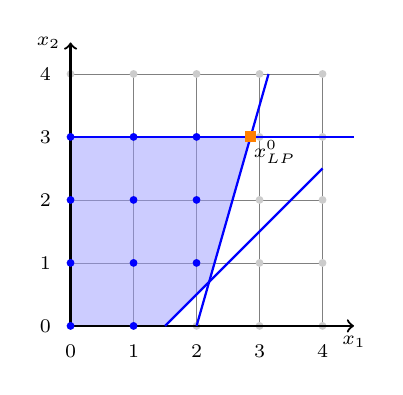
\begin{tikzpicture}[scale = 0.8,
			point/.style={circle, fill=gray!40, inner sep=1pt},
			feas point/.style={circle, fill=blue, inner sep=1pt}]
			\draw[help lines] (0,0) grid (4,4);  
			
			\fill[blue!40, opacity=0.5] (0,0) -- (1.5, 0) -- (2.2, 0.7) --(20/7, 3) -- (0,3);	
			\foreach \x in {0,...,4}{
			  \foreach \y in {0,...,4} {
			      \node[point] (\x,\y) at (\x, \y) {};
			  }}
			\foreach \x in {0,...,4}{
			  \node[font=\scriptsize] at (\x,-0.4) {$\x$};
			}
			\foreach \y in {0,...,4}{
			  \node[font=\scriptsize] at (-0.4,\y) {$\y$};
			}                      
			\draw[thick, <->] (4.5,0) node[below, font=\scriptsize]{$x_1$} -- (0,0) -- (0,4.5) node[left, font=\scriptsize]{$x_2$};    
			\draw[domain=0:4.5, thick, variable=\x, blue] plot ({\x},{3});
			\draw[domain=2:22/7, thick, variable=\x, blue] plot ({\x},{-14/2 + 7/2*\x});
			\draw[domain=1.5:4, thick,variable=\x,blue] plot ({\x},{-3/2 + \x});
			\node[fill=orange, inner sep=2pt] (LP) at (20/7, 3) {};          
			\node[font=\scriptsize, below right,inner sep=1pt] at (LP) {$x_{LP}^0$};
			\node[feas point] at (0,0){};
			\node[feas point] at (1,0){};
			\foreach \x in {0,...,2}{ 
			  \foreach \y in {1,...,3}{        
			      \node[feas point] at (\x,\y){};
			}}     
		\end{tikzpicture}
		\caption{}	
	\end{subfigure}
	\hfill
	\begin{subfigure}{0.32\textwidth}
		\centering
		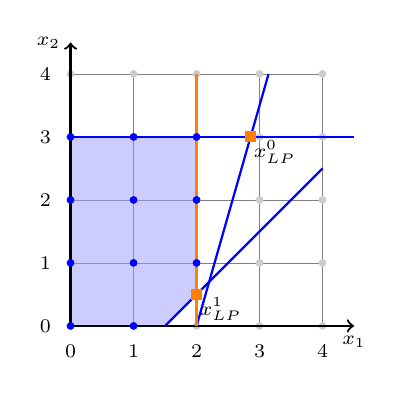
\begin{tikzpicture}[scale = 0.8,
          point/.style={circle, fill=gray!40, inner sep=1pt},
          feas point/.style={circle, fill=blue, inner sep=1pt}]
          \draw[help lines] (0,0) grid (4,4);  
          \fill[blue!40, opacity=0.5] (0,0) -- (1.5, 0) -- (2, 0.5) --(2, 3) -- (0,3);
          \foreach \x in {0,...,4}{
              \foreach \y in {0,...,4} {
                  \node[point] (\x,\y) at (\x, \y) {};
              }}
          \foreach \x in {0,...,4}{
              \node[font=\scriptsize] at (\x,-0.4) {$\x$};
          }
          \foreach \y in {0,...,4}{
              \node[font=\scriptsize] at (-0.4,\y) {$\y$};
          }                      
          \draw[thick, <->] (4.5,0) node[below, font=\scriptsize]{$x_1$} -- (0,0) -- (0,4.5) node[left, font=\scriptsize]{$x_2$};    
          \draw[domain=0:4.5, thick, variable=\x, blue] plot ({\x},{3});
          \draw[domain=2:22/7, thick, variable=\x, blue] plot ({\x},{-14/2 + 7/2*\x});
          \draw[domain=1.5:4, thick,variable=\x,blue] plot ({\x},{-3/2 + \x});
          \draw[orange, thick] (2,0) -- (2,4);
          \node[fill=orange, inner sep=2pt] (LP) at (20/7, 3) {};          
          \node[font=\scriptsize, below right,inner sep=1pt] at (LP) {$x_{LP}^0$};
          \node[fill=orange, inner sep=2pt] (LP) at (2, 1/2) {};          
          \node[font=\scriptsize, below right,inner sep=1pt] at (LP) {$x_{LP}^1$};
          \node[feas point] at (0,0){};
          \node[feas point] at (1,0){};
          \foreach \x in {0,...,2}{ 
              \foreach \y in {1,...,3}{        
                  \node[feas point] at (\x,\y){};
          }}
      \end{tikzpicture}
      \caption{}		
	\end{subfigure}
	\hfill
	\begin{subfigure}{0.32\textwidth}
		\centering
		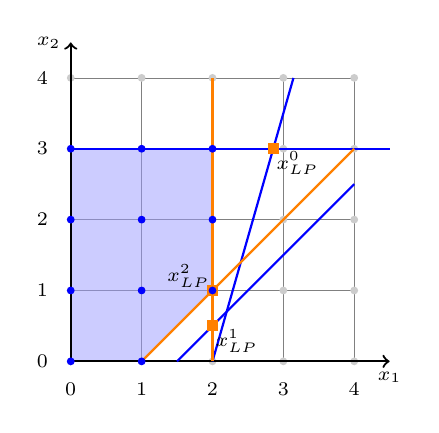
\begin{tikzpicture}[scale = 0.9,
          point/.style={circle, fill=gray!40, inner sep=1pt},
          feas point/.style={circle, fill=blue, inner sep=1pt}]
          \draw[help lines] (0,0) grid (4,4);  
          \fill[blue!40, opacity = 0.5] (0,0) -- (0,3) --(2,3) -- (2,1)	-- (1,0);
          \foreach \x in {0,...,4}{
              \foreach \y in {0,...,4} {
                  \node[point] (\x,\y) at (\x, \y) {};
              }}
          \foreach \x in {0,...,4}{
              \node[font=\scriptsize] at (\x,-0.4) {$\x$};
          }
          \foreach \y in {0,...,4}{
              \node[font=\scriptsize] at (-0.4,\y) {$\y$};
          }                      
          \draw[thick, <->] (4.5,0) node[below, font=\scriptsize]{$x_1$} -- (0,0) -- (0,4.5) node[left, font=\scriptsize]{$x_2$};    
          \draw[domain=0:4.5, thick, variable=\x, blue] plot ({\x},{3});
          \draw[domain=2:22/7, thick, variable=\x, blue] plot ({\x},{-14/2 + 7/2*\x});
          \draw[domain=1.5:4, thick, variable=\x,blue] plot ({\x},{-3/2 + \x});
          \draw[orange, thick] (2,0) -- (2,4);
          \draw[orange, thick] (1,0) -- (4,3);
          \node[fill=orange, inner sep=2pt] (LP) at (20/7, 3) {};          
          \node[font=\scriptsize, below right, inner sep=1pt] at (LP) {$x_{LP}^0$};
          \node[fill=orange, inner sep=2pt] (LP) at (2, 1/2) {};          
          \node[font=\scriptsize, below right, inner sep=1pt] at (LP) {$x_{LP}^1$};
          \node[fill=orange, inner sep=2pt] (LP) at (2, 1) {};          
          \node[font=\scriptsize, above left, inner sep=1pt] at (LP) {$x_{LP}^2$};
          \node[feas point] at (0,0){};
          \node[feas point] at (1,0){};
          \foreach \x in {0,...,2}{ 
              \foreach \y in {1,...,3}{        
                  \node[feas point] at (\x,\y){};
          }}         
      \end{tikzpicture}
      \caption{}		
	\end{subfigure}

      \caption{Feasible region of the LP relaxation (polyhedral set) and of the integer programming problem (blue dots) at each of three iterations taken to solve the integer programming problem. The inequalities in orange represent the Gomory cut added at each iteration} \label{p1c10:fig:LP_1}	
\end{figure}


\section{Obtaining stronger inequalities}

We finalise this chapter discussing the notion of strong inequalities and providing an example on how they can be made stronger in some cases by means of an external process. 


\subsection{Strong inequalities}

The notion of strong inequalities arises from the notion of stronger formulations, cf. Definition \ref{p1c8:def:better_formulations}. That is, we say that an inequality is strong in terms of its relative quality in describing the convex hull of integer set.

However, in this context we are interested in comparing two alternative inequalities to decide which is stronger. For that, we can rely on the notions of \emph{dominance} and related \emph{redundancy} of inequalities. 

Consider two valid inequalities $\pi x \leq \pi_0$ and $\mu x \leq \mu_0$ that are valid for a polyhedral set $P = \braces{x \in \reals^n_+ : Ax \leq b}$. Definition \ref{p1c10:def:dominance} formalises the notion of dominance.

\begin{definition}[Dominance] \label{p1c10:def:dominance}
    The inequality $\pi x \leq \pi_0$ \emph{dominates} $\mu x \leq \mu_0$ if these exists $u > 0$ such that $\pi \geq u\mu$, $\pi_0 \leq u\mu_0$, and $(\pi, \pi_0) \neq (u\mu, u\mu_0)$.
\end{definition}

Let us illustrate the concept of dominance with a numerical example. Consider the inequalities $2x_1 + 4x_2 \leq 9$ and $x_1 + 3x_2 \leq 4$, which are valid for $P = \conv(X)$, where 
	%
	\begin{equation*}
	X = \braces{(0,0), (0,1), (0,2), (0,3), (0,4), (1,0), (1,1)}.	
	\end{equation*}
	
Notice that, if we consider $u = 1/2$, we have that, for any $x=(x_1,x_2)$, that $1x_1 + 3x_2 \geq u(2x_1 + 4x_2) = x_1 + 2x_2$ and that $4 \leq 9u = 9/2$. Thus, we say that $x_1 + 3x_2 \le 4$ dominates $2x_1 + 4x_2 \leq 9$. Figure \ref{p1c10:fig:dominance} illustrates the two inequalities. Notice that $x_1 + 3x_2 \le 4$ is a stronger inequality, since it is more efficient in representing the convex hull of $X$ than $2x_1 + 4x_2 \le 9$.   

\begin{figure}
	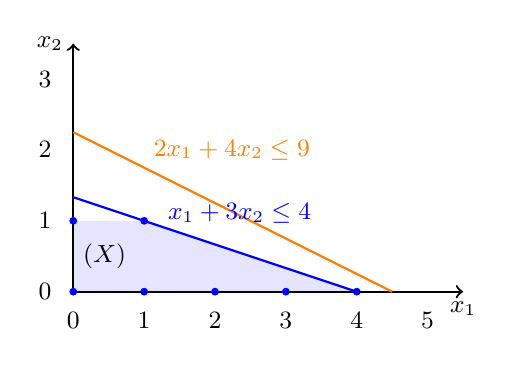
\begin{tikzpicture}[scale = 0.9,
		point/.style={circle, fill=gray!40, inner sep=1pt},
		feas point/.style={circle, fill=blue, inner sep=1pt}]
		\fill[blue!10] (0,0) -- (0,1) -- (1,1) -- (4,0) -- cycle;
		\foreach \x in {0,...,5}{
		  \node[font=\small] at (\x,-0.4) {$\x$};
		}
		\foreach \y in {0,...,3}{
		  \node[font=\small] at (-0.4,\y) {$\y$};
		}                      
		\draw[thick, <->] (5.5,0) node[below, font=\small]{$x_1$} -- (0,0) -- (0,3.5) node[left, font=\small]{$x_2$};    
		
		\draw[domain=0:4, thick, variable=\x, blue] plot ({\x},{-\x/3 + 4/3});
		\draw[domain=0:4.5, thick, variable=\x, orange] plot ({\x},{-\x/2 + 9/4});
		\node[feas point] at (2,0){};
		\node[feas point] at (3,0){};
		\node[feas point] at (4,0){};
		\foreach \x in {0,...,1}{ 
		  \foreach \y in {0,...,1}{        
		      \node[feas point] at (\x,\y){};
		}}
		\node [right,font=\small] at (1,2) {{\color{orange}$2x_1+4x_2 \leq 9$}};
		\node [right,font=\small] at (1.2,1.1) {{\color{blue}$x_1+3x_2 \leq 4$}};
		\node [right,font=\small] at (0,0.5) {$\conv(X)$};         
	\end{tikzpicture}
	\caption{Illustration of dominance between constraints. Notice that $x_1 + 3x_2 \le 4$ dominates $2x_1 + 4x_2 \le 9$ and is thus stronger}	\label{p1c10:fig:dominance}
\end{figure}

Another related concept is the notion of redundancy. Clearly, the presence of two constraints in which one dominates the other, the dominated constraint is also redundant and can be safely removed from the formulation of a polyhedral set $P$. However, in some cases one might not be able to identify redundant constraints simply because no constraint is clearly dominated by another. 

Even then, there might be a way to identify weak (or redundant) constraints by combining two or more constraints that then form a dominating constraint. This is formalised in Definition \ref{p1c10:def:redundancy}.

\begin{definition}[Redundancy] \label{p1c10:def:redundancy}
	The inequality $\pi x \leq \pi_0$ is \emph{redundant} for $P$ if there exists $k \geq 1$ valid inequalities $\pi^i x \leq \pi_0^i$ and $k\geq 1$ vectors $u_i > 0$, for $i \in \braces{1,\dots, k}$, such that $\left( \sum_{i=1}^k u_i\pi^i\right)x \leq \sum_{i=1}^ku_i\pi_0^i$ dominates $\pi x \leq \pi_0$.
\end{definition}

Once again, let us illustrate the concept with a numerical example. Consider we generate the inequality $5x_1 - 2x_2 \leq 6$, which is valid for the polyhedral set 
%
\begin{equation*}
	P = \braces{x \in \reals^2_+ : 6x_1 - x_2 \le 9, 9x_1 - 5x_2 \le 6}.
\end{equation*}
%
The inequality $5x_1 - 2x_2 \leq 6$ is not dominated by any of the inequalities forming $P$. However, if we set $u_i= (\frac{1}{3}, \frac{1}{3})$, we obtain $5x_1 - 2x_2 \leq 5$, which in turn dominates $5x_1 - 2x_2 \leq 6$. Thus, we can conclude that the generated inequality is redundant and does not improve the formulation of $P$. This is illustrated in Figure \ref{p1c10:fig:redundant}.

\begin{figure}[h]
	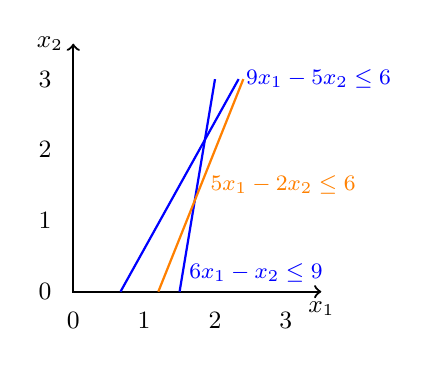
\begin{tikzpicture}[scale = 0.9,
	point/.style={circle, fill=gray!40, inner sep=1pt},
	feas point/.style={circle, fill=blue, inner sep=1pt}]
		\foreach \x in {0,...,3}{
		  \node[font=\small] at (\x,-0.4) {$\x$};
		}
		\foreach \y in {0,...,3}{
		  \node[font=\small] at (-0.4,\y) {$\y$};
		}                      
		\draw[thick, <->] (3.5,0) node[below, font=\small]{$x_1$} -- (0,0) -- (0,3.5) node[left, font=\small]{$x_2$};    
		\draw[domain=1.5:2, thick, variable=\x, blue] plot ({\x},{6*\x - 9});
		\draw[domain=2/3:7/3, thick, variable=\x, blue] plot ({\x},{9*\x/5 - 6/5});
		\draw[domain=6/5:12/5, thick, variable=\x, orange] plot ({\x},{2.5*\x - 3});       
		\node [above right,font=\footnotesize] at (1.5,0) {{\color{blue}$6x_1-x_2 \leq 9$}};
		\node [right,font=\footnotesize] at (2.3,3) {{\color{blue}$9x_1-5x_2 \leq 6$}};
		\node [right,font=\footnotesize] at (1.8,1.5) {{\color{orange}$5x_1-2x_2 \leq 6$}};
	\end{tikzpicture}
	\caption{Illustration of a redundant inequality. Notice how the inequality $5x_1 - 2x_2 \le 6$ (in orange) does not dominate any of the other inequalities} \label{p1c10:fig:redundant}
\end{figure}


As one might realise, checking whether a newly generated inequality improves the current formulation is a demanding task, as it requires finding the correct set of coefficients $u$ for all constraints currently forming the polyhedral set $P$. Nonetheless, the notions of redundancy and dominance can be used to guide procedures that generate or improve existing inequalities. Let us discuss one of such procedures, in the context of 0-1 knapsack inequalities.


\subsection{Strengthening 0-1 knapsack inequalities}

Let us consider the family of constraints known as knapsack constraints and see how they can be strengthened. For that, let us first define the knapsack set
%
\begin{equation*}
	X = \braces{x \in \braces{0,1}^n : \sum_{j=1}^n a_jx_j \leq b}.	
\end{equation*}
%
We assume that $a_j \geq 0$, $j \in N = \braces{1, \dots, n}$, and $b > 0$. Let us start by defining the notion of a \emph{minimal cover}.

\begin{definition} [minimal cover] \label{p1c10:def:minimal_cover}
	A set $C \subseteq N$ is a cover if $\sum_{j \in C} a_j > b$. A cover $C$ is minimal if $C \setminus \braces{j}$ for all $j \in C$ is not a cover.  
\end{definition} 

Notice that a cover $C$ refers to any selection of items that exceed the budget $b$ of the constraint and this selection is said to be a minimal cover if, upon removing of any item of the selection, the constraint becomes satisfied. This logic allows us to design a way to generate valid inequalities using covers. This is the main result in Proposition \ref{p1c10:prop:cover_inequalities}.

\begin{proposition} \label{p1c10:prop:cover_inequalities}
	If $C \subseteq N$ is a cover for $X$, then a valid cover inequality for $X$ is
	% 
	\begin{equation*}
		\sum_{j \in C} x_j \leq |C|-1.		
	\end{equation*}
\end{proposition}

\begin{proof} 
	Let $R = \braces{j \in N : x^R_j = 1}$, for $x^R \in X$. If $\sum_{j \in C}x_j^R > |C|-1$, then $|R \cap C| = |C|$ and $C \subseteq R$. Thus, $\sum_{j\in N}a_j x_j^R = \sum_{j\in R}a_j > b$, which violates the inequality and implies that $x^R \notin X$.  
\end{proof}

The usefulness of Proposition \ref{p1c10:prop:cover_inequalities} becomes evident if $C$ is a minimal cover. Let us consider a numerical example to illustrate this. Consider the knapsack set 
%
\begin{equation*}
	X = \braces{x \in \braces{0,1}^7 : 11x_1 + 6x_2 + 6x_3 + 5x_4 + 5x_5 + 4x_6 + x_7 \leq 19}.	
\end{equation*}

The following are minimal cover inequalities for $X$. 
%
\begin{align*}
&x_1 + x_2 + x_3 \leq 2\\
&x_1 + x_2 +x_6 \leq 2\\
&x_1 + x_5 + x_6 \leq 2\\
&x_3 + x_4 + x_5 + x_6 \leq 3
\end{align*}

Notice that we would obtain a non-minimal cover $C^\prime$ by adding an inequality $x_i \leq 1$, $i \in C^\prime\setminus C$, to a minimal cover inequality of $C$, which makes the cover inequality somewhat redundant. For example, adding $x_7 \leq 1$ to a minimal cover inequality $x_1 + x_2 + x_3 \leq 2$ of $C = \{1,2,3\}$ yields a non-minimal cover $C^\prime = \braces{1,2,3,7}$ with inequality $x_1 + x_2 + x_3 + x_7 \leq 3$.

There is a simple way to strengthen cover inequalities, using the the notion of \emph{extended} cover inequalities. One can extend a cover inequality by expanding the set $C$ with elements that have a coefficient $a_j$, $j \in N \setminus C$ greater or equal than all coefficients $a_i$, $i \in C$. This guarantees that a swap between elements must happen for the inequality to be feasible, meaning that the righthand side of the constraint remains $|C| - 1$. This is summarised in Proposition \ref{p1c10:prop:extended_cover}.

\begin{proposition} \label{p1c10:prop:extended_cover}
	If $C$ is a cover for $X$, the extended cover inequality
	%
	\begin{equation*}
		\sum_{j \in E(C)} x_j \leq |C|-1
	\end{equation*}
	% 
	with $E(C) = C \cup \braces{j\in N: a_j \geq a_i, \forall i \in C}$ is valid for $X$.
\end{proposition}

We leave the proof as a thought exercise. Let us however illustrate this using the previous numerical example. For $C = \braces{3,4,5,6}$, $E(C) = \braces{1,2,3,4,5,6}$, yielding the inequality 
%
\begin{equation*}
	x_1 + x_2 + x_3 + x_4 + x_5 + x_6 \leq 3	
\end{equation*}
%
which is stronger than $x_3 + x_4 + x_5 + x_6 \leq 3$ as the former dominates the latter, cf. Definition \ref{p1c10:def:dominance}. 


\section{Exercises}

\subsection*{Exercise 10.1: Chv\'atal-Gomory (C-G) procedure}
Consider the set $X = P \cap \integers^n$ where $P = \{x \in \reals^n : Ax \leq b, x\geq 0 \}$ and in which $A$ is an $m \times n$ matrix with columns $\{A_1, \dots, A_n\}$. Let $u \in \reals^m$ with $u\geq 0$. The Chvátal-Gomory (C-G) procedure to construct valid inequalities for $X$ uses the following 3 steps:
    \begin{enumerate}
        \item $\sum\limits_{j=1}^n uA_jx_j \leq ub$ is valid for $P$, as $u\geq 0$ and $\sum\limits_{j=1}^n A_jx_j \leq b$.
        \item $\sum\limits_{j=1}^n \floor{uA_j}x_j \leq ub$ is valid for $P$, as $x \geq 0$.
        \item $\sum\limits_{j=1}^n  \floor{uA_j}x_j \leq \floor{ub}$ is valid for $X$, as any $x\in X$ is integer and thus $\sum\limits_{j=1}^n\floor{uA_j}x_j$ is integer.
    \end{enumerate}
Show that every valid inequality for $X$ can be obtained by applying the Chvátal-Gomory procedure a finite number of times.

\emph{Hint:} We show this for the 0-1 case. Thus, let $P = \{x\in \reals^n : Ax\leq b, 0\leq x \leq 1\}$, $X = P \cap \integers^n$, and suppose that $\pi x \leq \pi_0$ with $\pi,\pi_0\in \integers$ is a valid inequality for $X$. We show that $\pi x \leq \pi_0$ can be obtained by applying Chvátal-Gomory procedure a finite number of times. We do this in parts by proving the following claims \textbf{C1}, \textbf{C2}, \textbf{C3}, \textbf{C4}, and \textbf{C5}.\\

\textbf{C1.} An inequality $\pi x \leq \pi_0 + t$ with $t\in \integers_+$ is valid for $P$.\\

\textbf{C2.} For a large enough $M\in \integers_+$, the inequality 
\begin{equation}\label{eq:M}
\pi x \leq \pi_0 + M\bigg{(}\sum_{j\in N^0}x_j + \sum_{j\in N^1}(1-x_j)\bigg{)}
\end{equation}
is valid for $P$ for every partition $(N^0,N^1)$ of $N$.\\

\textbf{C3.} If $\pi x \leq \pi_0 + \tau + 1$ is a valid inequality for $X$ with $\tau\in \integers_+$, then
\begin{equation}\label{eq:tau}
\pi x \leq \pi_0 + \tau + \sum_{j\in N^0} x_j + \sum_{j\in N^1}(1-x_j)
\end{equation}
is also a valid inequality for $X$ for every partition $(N^0,N^1)$ of $N$.\\

\textbf{C4.} If 
\begin{equation}\label{eq:41}
\pi x \leq \pi_0 + \tau + \sum_{j\in T^0\cup \{p\}} x_j + \sum_{j\in T^1} (1-x_j)
\end{equation}
and 
\begin{equation}\label{eq:42}
\pi x \leq \pi_0 + \tau + \sum_{j\in T^0} x_j + \sum_{j\in T^1\cup \{p\}} (1-x_j)
\end{equation}
are valid inequalities for $X$, where $\tau \in \integers_+$ and $(T^0,T^1)$ is any partition of $\{1,\dots,p-1\}$, then
\begin{equation}\label{eq:C4}
\pi x \leq \pi_0 + \tau + \sum_{j\in T^0} x_j + \sum_{j\in T^1} (1-x_j)
\end{equation}
is also a valid inequality for $X$.\\

\textbf{C5.} If 
\begin{equation}\label{eq:C51}
\pi x \leq \pi_0 + \tau + 1
\end{equation}
is a valid inequality for $X$ with $\tau \in \integers_+$, then
\begin{equation}\label{eq:C52}
\pi x \leq \pi_0 + \tau
\end{equation}
is also a valid inequality for $X$.

Finally, after proving the claims \textbf{C1} - \textbf{C5}, if we start with $\tau = t-1 \in \integers_+$ and successively apply \textbf{C5} for $\tau = t-1,\dots,0$, turning each valid inequality \eqref{eq:C51} of $X$ into a new one \eqref{eq:C52}, it leads to the inequality $\pi x\leq \pi_0$ which is valid for $X$. This shows that every valid inequality $\pi x \leq \pi_0$ of $X$ with $\pi,\pi_0\in \integers_+$ can be obtained by applying the C-G procedure a finite number of times. 

\subsection*{Exercise 10.2: Chv\'atal-Gomory (C-G) procedure example}
\begin{enumerate}
\item[(a)] Consider the set $X = \{\mathbf{x} \in \mathbb{B}^5 : 3x_1 - 4x_2 + 2x_3 - 3x_4 + x_5 \leq -2 \}$. Derive the following inequalities as C-G inequalities:
\begin{enumerate}
\item[($i$)] $x_2 + x_4 \geq 1$
\item[($ii$)] $x_1 \leq x_2$
\end{enumerate}
\item[(b)] Consider the set $X = \{x \in \mathbb{B}^4 : x_i + x_j \leq 1 \textrm{ for all } i,j\in \{1,\dots,4\} : i\neq j\}$. Derive the clique inequalities $x_1 + x_2 + x_3 \leq 1$ and $x_1+ x_2 + x_3 + x_4 \leq 1$ as C-G inequalities.
\end{enumerate}



\subsection*{Exercise 10.3: Cuts from the simplex tableau}
Consider the integer programming problem $IP$:
\begin{align*}
(IP) \quad \maxi_{x_1,x_2} \quad  & 2x_1+5x_2 \\
\st   ~~ & 4x_1 + x_2 \leq 28 \\
      & x_1 + 4x_2 \leq 27 \\
      & x_1-x_2 \leq 1\\
      & x_1,x_2 \in \integers_+.
\end{align*}
The LP relaxation of the problem $IP$ is obtained by relaxing the integrality constraints $x_1,x_2\in \integers_+$ to $x_1 \geq 0$ and $x_2 \geq 0$. The LP relaxation of $IP$ in standard form is the problem $LP$:
\begin{align*}
(LP) \quad \maxi_{x_1,x_2} \quad  & 2x_1+5x_2 \\
\st   ~~ & 4x_1 + x_2 + x_3 = 28\\
      & x_1 + 4x_2 + x_4 = 27\\
      & x_1-x_2 + x_5  =  1\\
      & x_1,x_2,x_3,x_4,x_5\geq 0
\end{align*}
The optimal Simplex tableau after solving the problem $LP$ with primal Simplex is
\renewcommand*{\arraystretch}{1.2}
\[
\begin{tabular}{ccccc|c}
       $x_1$& $x_2$ & $x_3$ & $x_4$ & $x_5$ & RHS  \\
\hline
      0 & 0 & -1/5  & -6/5 & 0   & -38 \\
\hline
      1 & 0 & 4/15  & -1/15 & 0 & 17/3 \\
      0 & 1 & -1/15 & 4/15  & 0 & 16/3 \\
      0 & 0 & -1/3  & 1/3   & 1 & 2/3
\end{tabular}
\]

\begin{itemize}
\item[(a)] Derive two fractional Gomory cuts from the rows of $x_1$ and $x_5$, and express them in terms of the original variables $x_1$ and $x_2$.
\item[(b)] Derive the same cuts as in part (a) as Chv\'{a}tal-Gomory cuts. \emph{Hint:} Use Proposition 5 from \href{https://mycourses.aalto.fi/mod/folder/view.php?id=651663}{Lecture 9}. Recall that the bottom-right part of the tableau corresponds to $B^{-1}A$, where $B^{-1}$ is the inverse of the optimal basis matrix and $A$ is the original constraint matrix. You can thus obtain the matrix $B^{-1}$ from the optimal Simplex tableau, since the last three columns of $A$ form an identity matrix.
\end{itemize}

\subsection*{Exercise 10.4: More Gomory cuts}
Consider the following integer programming problem $IP$:

\begin{align*}
	(IP) : \maxi z =~& x_1 + 2x_2   \\
	\st & -3x_1 + 4x_2 \le 4 \\
		& 3x_1 + 2x_2 \le 11 \\
		& 2x_1 - x_2 \le 5   \\
		& x_1, x_2 \in \integers_+
\end{align*}

Solve the problem by adding Gomory cuts to the LP relaxation until you find an integer solution.

\subsection*{Exercise 10.5. The cover separation problem}
Consider the 0-1 knapsack set :

$$X = \braces{x \in \braces{0,1}^7 : 11x_1 + 6x_2 + 6x_3 + 5x_4 + 5x_5 + 4x_6 + x_7 \leq 19}$$

and a solution $\bar{x} = (0, 2/3, 0, 1, 1, 1, 1)$ to its LP relaxation. Find a cover inequality cutting out (violated by) the fractional solution $\bar{x}$.



